\documentclass{article}
\usepackage{graphicx} % Required for inserting images
\usepackage{float}
\usepackage[T1]{fontenc}
\usepackage{amsmath}
\usepackage[margin=1in]{geometry}
\usepackage{booktabs}
\usepackage{tabularx}
\usepackage[hidelinks]{hyperref}

\title{Forecasting 22-day SPY volatility: HAR, HAR-X and a random forest against GARCH}
\author{Experiment report \textperiodcentered{} L/S Gamma Desk, QUANTT}
\date{2026-10-18}

\begin{document}

\maketitle

\textbf{Question:} Do HAR on Garman-Klass RV (\texttt{har\_\allowbreak{}gk}), HAR-X (adding VIX and last week's return, \texttt{harx}) and a random forest on the HAR-X inputs (\texttt{rf}) each forecast SPY's 22-day realized variance better than the live GARCH(1,1) on QLIKE, with a smaller calm-day bias, in each of 2000-2013, 2014-2019 and 2020-2024?

\textbf{Method:}

\begin{itemize}

\item \textbf{Pre-registration:} the card was committed before the run (commit b5f5413). The research-only forecasters were committed just before it (a69142b).

\item \textbf{Card 1 of 2:} this one tests forecast accuracy only. Card 2 would put any passer into the option backtest's signal.

\item \textbf{Data:} the backtest's completed-day features (SPY daily from CRSP, Garman-Klass RV from the daily open, high, low and close, VIX from CBOE). Every input is also in the live pipeline.

\item \textbf{Forecast dates:} 6,267 trading days from 2000-01-03, ending where the 22-day target window would reach the hold-out (2025-01-01), which was not used.

\item \textbf{Target:} the mean squared daily log return over the next 22 trading days. A forecast at the close of day t uses completed days up to t.

\item \textbf{Reference:} the live GARCH(1,1), refit every day on the trailing 5 years of returns, as it runs live.

\item \textbf{Candidates:}

\begin{itemize}

\item \texttt{har\_\allowbreak{}gk}: a direct 22-day regression on daily, weekly and monthly Garman-Klass RV.

\item \texttt{harx}: the same, plus VIX and last week's return.

\item \texttt{rf}: a random forest on the \texttt{harx} inputs, with 300 trees and at least 20 rows per leaf, fixed before the run.

\end{itemize}

\item \textbf{Walk-forward:} the candidates refit on the first trading day of each month, on the trailing 5 years, using only rows whose target was complete. Between refits they forecast daily from the newest completed day.

\end{itemize}

This report was written by Claude at the PM's request.

\section{Result vs the pass bar}

Each candidate had to hold both checks in every period:

\begin{itemize}

\item a lower mean QLIKE than GARCH (lower is better);

\item a smaller absolute median calm-day bias, i.e. forecast minus realized vol in vol points, on days when the completed-day VIX was below 20.

\end{itemize}

The event floor was 250 calm days per period. Every period met it, with 1,841, 1,341 and 633 calm days.

\begin{center}\small
\begin{tabularx}{\linewidth}{l >{\raggedright\arraybackslash}X l l l l}
\toprule
\textbf{Period} & \textbf{Check} & \textbf{GARCH} & \textbf{har\_gk} & \textbf{harx} & \textbf{rf} \\
\midrule
2000-2013 & QLIKE & 0.264 & 0.795 fail & 0.379 fail & 0.365 fail \\
2000-2013 & calm-day bias & +2.28 & +5.83 fail & +2.68 fail & +1.52 pass \\
2014-2019 & QLIKE & 0.369 & 0.364 pass & 0.348 pass & 0.407 fail \\
2014-2019 & calm-day bias & +3.12 & +3.50 fail & +2.55 pass & +1.77 pass \\
2020-2024 & QLIKE & 0.538 & 0.684 fail & 0.802 fail & 0.753 fail \\
2020-2024 & calm-day bias & +3.17 & +5.79 fail & +4.34 fail & +3.94 fail \\
\bottomrule
\end{tabularx}
\end{center}

\textbf{Verdict: failed for all three candidates.} No candidate holds both checks in more than one period. All three fail both checks in 2020-2024. So card 2 (P\&L) has no forecaster to test, and live stays on GARCH.

\subsection{Full-window numbers (not part of the bar)}

\begin{center}\small
\begin{tabularx}{\linewidth}{>{\raggedright\arraybackslash}X l l l l}
\toprule
\textbf{2000-2024} & \textbf{GARCH} & \textbf{har\_gk} & \textbf{harx} & \textbf{rf} \\
\midrule
Mean QLIKE & 0.343 & 0.669 & 0.455 & 0.452 \\
Newey-West t of QLIKE gap vs GARCH &  & +2.4 & +3.0 & +2.1 \\
Median calm-day bias (vol pts) & +2.68 & +4.68 & +2.89 & +1.90 \\
Median bias, all days (vol pts) & +2.40 & +3.71 & +2.70 & +1.79 \\
Mean bias, all days (vol pts) & +1.13 & +1.88 & +1.60 & +1.01 \\
Forecasts at the 5\% floor & 0 & 0 & 45 & 0 \\
\bottomrule
\end{tabularx}
\end{center}

A positive t means the candidate's loss is higher than GARCH's. Over the full window all three are significantly worse, with t above 2. The two QLIKE wins, both in 2014-2019, are not significant: \texttt{har\_\allowbreak{}gk} has t = \ensuremath{-}0.6 and \texttt{harx} t = \ensuremath{-}1.0. \texttt{harx} hit the 5\% floor 45 times: 37 in 2000-2013 and 8 in 2020-2024.

\section{Charts}

\begin{figure}[H]\centering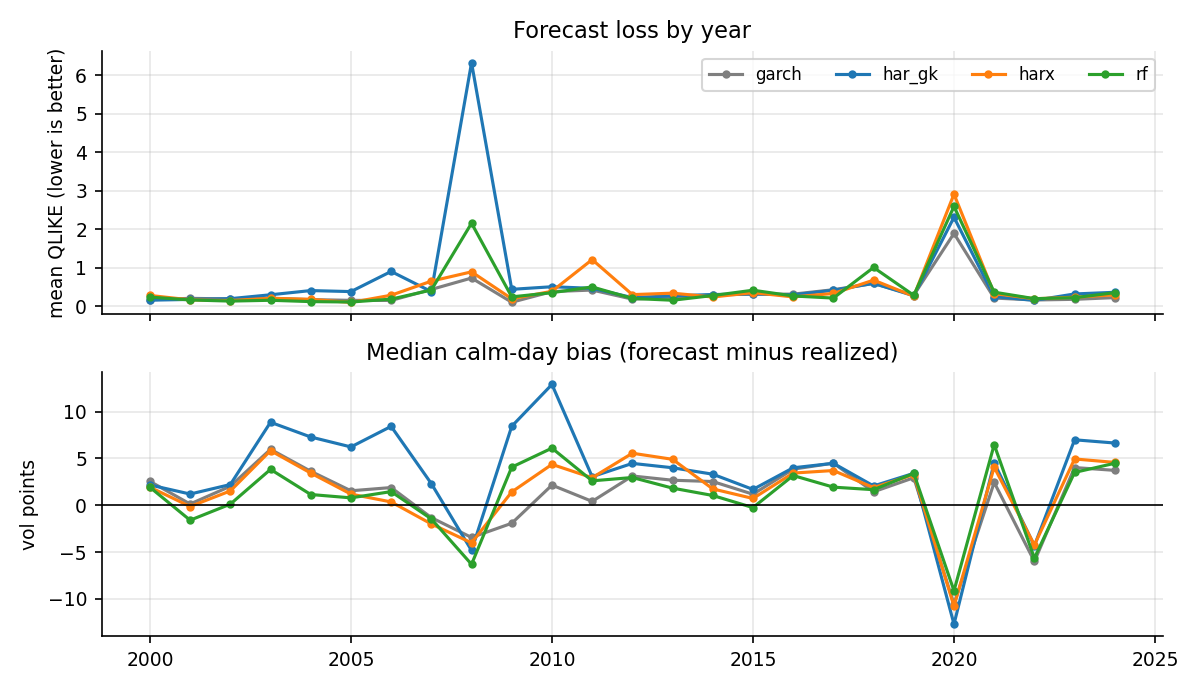
\includegraphics[width=0.92\linewidth]{figures/yearly.png}\caption{QLIKE and median calm-day bias by year}\end{figure}

The top panel shows that the losses come from a few years. Each candidate's QLIKE is close to GARCH's in most years and jumps in 2008 and 2020; \texttt{har\_\allowbreak{}gk} reaches 6.3 in 2008. The bottom panel shows the calm-day bias. The random forest sits below GARCH in most years before 2020, except 2009-2011, 2018 and 2019. After 2020 every candidate is above GARCH in 2021, 2023 and 2024, apart from \texttt{rf} in 2023.

\begin{figure}[H]\centering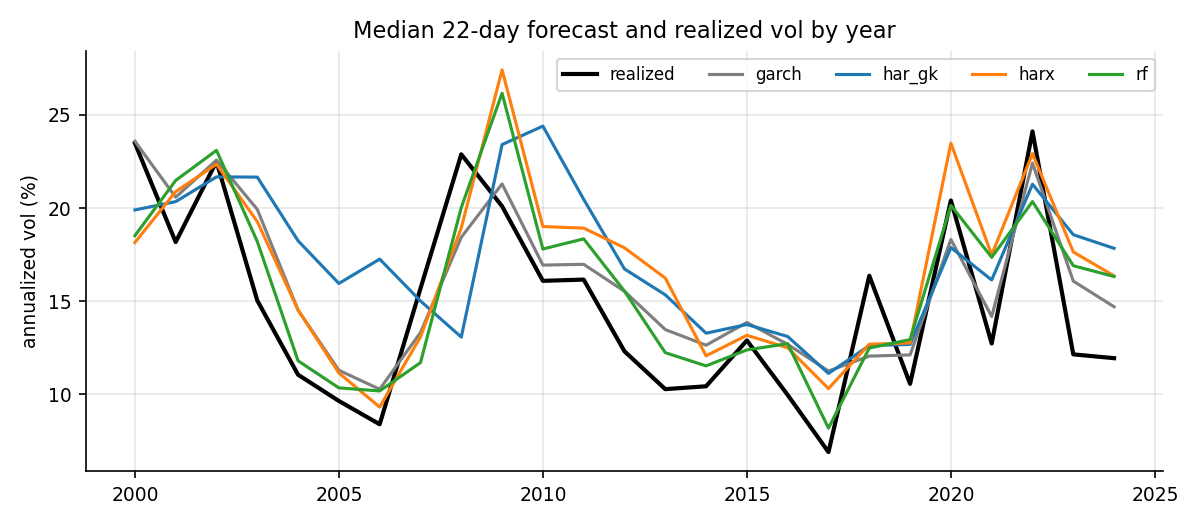
\includegraphics[width=0.92\linewidth]{figures/levels.png}\caption{Median 22-day forecast and realized vol by year}\end{figure}

All four models forecast above the median realized vol in most years, including every calm one (for example 2004-2006, 2012-2014, 2016-2017, 2019, 2021 and 2023-2024). \texttt{har\_\allowbreak{}gk} runs above the others in 2010-2011 and below realized in 2007-2008, for the data reason explained below.

\begin{figure}[H]\centering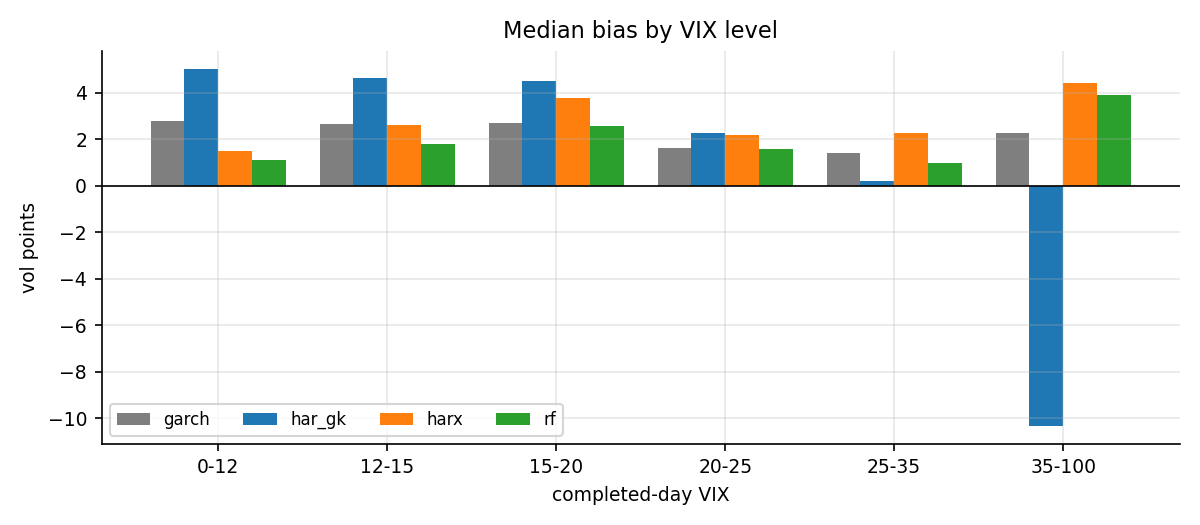
\includegraphics[width=0.92\linewidth]{figures/by_vix.png}\caption{Median bias by VIX level}\end{figure}

Below VIX 12, the random forest and HAR-X are less biased than GARCH (1.1 and 1.5 points against 2.8). Between VIX 12 and 20 only the random forest is clearly less biased (1.8 against 2.6, and 2.6 against 2.7); HAR-X ties GARCH from 12 to 15 and is worse from 15 to 20. Above VIX 35, \texttt{har\_\allowbreak{}gk} forecasts far too low.

\section{Analysis}

\begin{itemize}

\item \textbf{GARCH wins in the spikes, and the spikes dominate QLIKE.}

\begin{itemize}

\item \textbf{Losses concentrate in a few days.} QLIKE punishes forecasts that are too low much more than forecasts that are too high. The worst 5\% of days make up 47\% of GARCH's total loss and 55-59\% of each candidate's.

\item \textbf{2020 shows the gap.} From 20 February to 15 April 2020 the median realized vol was 56.1\%. GARCH forecast a median 46.3\%, the candidates 22-29\%. GARCH refits daily, and its variance updates with every new squared return. The candidates' coefficients stay fixed for a month.

\item \textbf{The random forest has a hard ceiling.} It can't forecast above the largest target in its training window. Its highest forecast in that stretch of 2020 was 26.2\%.

\item \textbf{Excluding the crisis years doesn't save the candidates} (a check made after the run). Without 2008 and 2020, GARCH still has the lowest QLIKE in 2020-2024: 0.191 against 0.26-0.28.

\end{itemize}

\item \textbf{The random forest cuts calm-day bias but not after 2020.}

\begin{itemize}

\item \textbf{Before 2020 it is the least biased model.} Its median calm-day bias is +1.5 points in 2000-2013 and +1.8 in 2014-2019, against GARCH's +2.3 and +3.1. \texttt{harx} also beats GARCH in 2014-2019.

\item \textbf{From 2021 every candidate runs higher than GARCH,} apart from \texttt{rf} in 2023. In 2021 the random forest is at +6.5 against +2.4, and in 2023-2024 \texttt{har\_\allowbreak{}gk} is at +7.0 and +6.7. With the 2020 crash in their 5-year training window, the regressions forecast high in the calm years after it. The live HAR showed the same pattern in \texttt{2026-\allowbreak{}10-\allowbreak{}16-\allowbreak{}har-\allowbreak{}signal}.

\end{itemize}

\item \textbf{Part of the ``calm-day bias'' is skew, not error.} Realized vol is right-skewed: most calm months are quieter than average, and a few calm days are followed by a spike. A forecast of expected variance should therefore sit above the typical calm month.

\begin{itemize}

\item \textbf{2020-2024 shows the split.} On calm days GARCH's median vol bias was +3.2 points, but its mean forecast variance was only 0.85 of the mean realized variance. So on average it was too \emph{low}.

\item \textbf{Cutting median bias costs elsewhere.} A model lowers its median bias mostly by forecasting below expected variance, and that is the error QLIKE punishes in spikes. The random forest shows the trade-off: the lowest median bias, and worse QLIKE than GARCH in all three periods. \texttt{2026-\allowbreak{}10-\allowbreak{}07-\allowbreak{}garch-\allowbreak{}bias-\allowbreak{}correction} found the same with a bias-corrected GARCH.

\end{itemize}

\item \textbf{A bad data point broke \texttt{har\_\allowbreak{}gk} in 2006-2011.}

\begin{itemize}

\item \textbf{The print.} The features file has one Garman-Klass value of 899\% annualized vol, on 2006-01-26, a day when SPY moved 0.55\%. It is the only day from 1993 to 2024 above 150\%. It looks like a bad daily high or low in the source data.

\item \textbf{What it did.} From the April 2006 refit to the January 2011 refit, that one point pushes the regression coefficients of \texttt{har\_\allowbreak{}gk} to about zero (the February 2011 refit is still distorted). Its forecast is then roughly constant. Checked after the run: on the refit of 1 October 2008, the forecast for 10 October was 13.6\% with the bad print and 64.2\% with that day's value replaced by its squared return. This explains \texttt{har\_\allowbreak{}gk}'s collapse in 2008 (median forecast 13.6\% against 74.0\% realized, 15 September to 30 November) and its high forecasts in 2009-2011.

\item \textbf{On clean data every candidate still fails 2000-2013.} After the run, the point was replaced by that day's squared return and the candidates refit for January 2006 to March 2011. 2000-2013 QLIKE is then 0.303 for \texttt{har\_\allowbreak{}gk} (0.795 as run), 0.519 for \texttt{harx} (0.379 as run) and 0.362 for \texttt{rf} (0.365), against GARCH's 0.264. \texttt{har\_\allowbreak{}gk}'s 2008 QLIKE falls from 6.3 to 0.75, close to GARCH's 0.73. The random forest's stays at 2.13: its 2008 loss is the training-range ceiling, not the print. (Dropping the whole window, 27 January 2006 to 31 January 2011, makes the random forest look better than GARCH, 0.194 against 0.212. But that only works because it drops 2008.)

\item \textbf{The verdict doesn't depend on it.} The 2014-2019 and 2020-2024 training windows start from 2009, after the last affected refit, and every candidate fails 2020-2024 on both checks.

\item \textbf{The rest of the desk is not affected.} The live signal and the option backtest use GARCH on close-to-close returns, which doesn't read the Garman-Klass column. Live uses yfinance.

\end{itemize}

\end{itemize}

\section{Verdict}

\textbf{Failed} for all three candidates on the pre-registered bar. The pass bar was not changed. Card 2 (P\&L) is not run, because no forecaster passed. GARCH stays the live forecaster.

What this means for the desk: on this evidence, a better forecast won't fix the signal's calm-stretch problem. GARCH is the hardest of the four to beat where it matters for QLIKE, in the spikes. The calm-day bias that keeps the signal flat is partly the skew of realized vol, which any honest forecast of expected variance carries. Possible follow-ups, each needing its own card:

\begin{itemize}

\item \textbf{Fix the Garman-Klass print} in the backtest's daily data, with a validation rule such as a cap relative to close-to-close variance, before any model reads the Garman-Klass column again. The history build is shared tooling, so this is a PM decision.

\item \textbf{A log-HAR fitted daily} (regression on log RV, the standard fix for heavy tails) might help with both failure modes here: slow reaction in spikes and sensitivity to outliers. It is the most defensible next rung if the desk keeps going.

\item \textbf{Change the signal, not the forecast.} If the signal compares IV with a median-type forecast rather than expected variance, it would go short more often in calm stretches. That is a signal-design test on the P\&L backtest. It is close to always-short, so its value over \texttt{2026-\allowbreak{}10-\allowbreak{}17-\allowbreak{}always-\allowbreak{}short} should be stated up front.

\end{itemize}

\section{Caveats}

\begin{itemize}

\item \textbf{Forecast accuracy is not P\&L.} The OPHR paper (in the desk's library) and \texttt{2026-\allowbreak{}10-\allowbreak{}16-\allowbreak{}har-\allowbreak{}signal} show the two can disagree. This card only settles that no candidate is a clear forecast improvement.

\item \textbf{Overlapping targets:} daily forecasts of 22-day windows overlap. The Newey-West t-statistics allow for this, but each period has fewer independent observations than its day count suggests.

\item \textbf{The bad print:} it distorts \texttt{har\_\allowbreak{}gk} in 2000-2013, as quantified above, but no candidate passes that period on clean data either. The other periods are clean.

\item \textbf{Calm days:} a completed-day VIX below 20, as pre-registered. 2020 and 2022 have few calm days (35 and 23), so 2020-2024's calm bias rests mostly on 2021, 2023 and 2024.

\item \textbf{Fixed design choices:} the monthly refit, the 5-year window and the random-forest settings were set before the run. Faster refits or other windows might change the ranking, and each change would be a new trial.

\item \textbf{Hold-out:} not used. In the replay features, Garman-Klass RV is zero from 2026-01-02 (parity closes have no high or low), so a hold-out test would also need a fallback.

\end{itemize}

\section{Trials}

One run of \texttt{experiment.\allowbreak{}py} at commit b5f5413, scoring three candidates against the GARCH reference: 3 trials. Forecast-only runs are logged under the experiment's results folder, not in the option backtest's registry. The post-hoc checks above (excluding 2008 and 2020, excluding the affected window, refitting the candidates for 2006-2011 without the bad print) read the saved forecasts or refit the same three candidates on corrected data. None is a new candidate, and they add no trials. After the run, the first figure was made shorter for layout and rebuilt with \texttt{-\allowbreak{}-\allowbreak{}report-\allowbreak{}only}. The pass bar was not changed.

\end{document}
